%T21: 2, 4, 7, 11, 14, 20, hillier (13 in reference paper)

\documentclass[twoside]{article}
\usepackage{fontspec}
\setromanfont[BoldFont={GenBasB.ttf},ItalicFont={GenBasI.ttf},BoldItalicFont={GenBasBI.ttf}]{GenBasR.ttf}
\usepackage{lipsum} % Package to generate dummy text throughout this template
\renewcommand\refname{\textbf{References}}
\linespread{1.00} % Line spacing - Palatino needs more space between lines
\usepackage{microtype} % Slightly tweak font spacing for aesthetics

\usepackage[hmarginratio=1:1,top=30mm, left=20mm, columnsep=20pt]{geometry} % Document margins
\usepackage{multicol} % Used for the two-column layout of the document
\usepackage[hang, small,labelfont=bf,up,textfont=it,up]{caption} % Custom captions under/above floats in tables or figures
\usepackage{booktabs} % Horizontal rules in tables
\usepackage{float} % Required for tables and figures in the multi-column environment - they need to be placed in specific locations with the [H] (e.g. \begin{table}[H])
\usepackage{hyperref} % For hyperlinks in the PDF

\usepackage{lettrine} % The lettrine is the first enlarged letter at the beginning of the text
\usepackage{paralist} % Used for the compactitem environment which makes bullet points with less space between them

\usepackage{abstract} % Allows abstract customization
\renewcommand{\abstractnamefont}{\normalfont\bfseries} % Set the "Abstract" text to bold
\renewcommand{\abstracttextfont}{\normalfont\small\itshape} % Set the abstract itself to small italic text

\usepackage{titlesec} % Allows customization of titles
\renewcommand\thesection{\arabic{section}} % Roman numerals for the sections
\renewcommand\thesubsection{\arabic{section}.\arabic{subsection}} % Arabic numerals for subsections
\titleformat{\section}[block]{\large\centering}{\textbf{\thesection.}}{1em}{} % Change the look of the section titles
\titleformat{\subsection}[block]{}{\textbf{\thesubsection}}{1em}{} % Change the look of the section titles

\usepackage{fancyhdr} % Headers and footers
\pagestyle{fancy} % All pages have headers and footers
\fancyhead{} % Blank out the default header
\fancyfoot{} % Blank out the default footer
\fancyhead[C]{\textit{S. Vermassen and T. Vervack. The performance of queueing networks with blocking (2014).}} % Custom header text
\fancyfoot[RO,LE]{\thepage} % Custom footer text

%----------------------------------------------------------------------------------------
%	TITLE SECTION
%----------------------------------------------------------------------------------------

\title{\vspace{-15mm}\fontsize{24pt}{10pt}\selectfont\textbf{The performance of queueing networks with blocking: a survey paper}} % Article title

\author{
\large
\textsc{Stefaan Vermassen \& Titouan Vervack}\\[2mm] 
\normalsize Ghent University \\ 
\normalsize \href{mailto:Stefaan.Vermassen@UGent.be}{Stefaan.Vermassen@UGent.be} \\
\normalsize \href{mailto:Titouan.Vervack@UGent.be}{Titouan.Vervack@UGent.be} 
\vspace{-5mm}
}
\date{}

%----------------------------------------------------------------------------------------

\begin{document}

\maketitle % Insert title

\thispagestyle{fancy} % All pages have headers and footers

%----------------------------------------------------------------------------------------
%	ABSTRACT
%----------------------------------------------------------------------------------------

\begin{abstract}

This review presents a comprehensive survey on queueing modeling issues and the related performance evaluation and optimization of queueing networks with blocking. To provide a systematic review of current relevant research, a classification scheme is proposed with regard to the key parameters in the network (single- or multiserver configurations, topology, and so on) and the related performance evaluation and optimization approaches. Secondly,  it presents ideas for future research by identifying gaps in the current literature.\\\\
\textbf{Keywords:} Queueing networks, Blocking, Performance evaluation and optimization, Generalized expansion method
\end{abstract}
\vspace{12mm}
%----------------------------------------------------------------------------------------
%	ARTICLE CONTENTS
%----------------------------------------------------------------------------------------

\begin{multicols}{2} % Two-column layout throughout the main article text

\section{\textbf{Introduction}}

\lettrine[nindent=0em,lines=3]{T}he evaluation and design of general service, finite waiting room, multi-server queueing networks with blocking is a complex optimization problem.  Queueing modelling and optimization for the performance assessment of complex manufacturing systems and production lines have been and continue to be the focus of several studies over the past decades.
\\\\
The aim of this survey paper is twofold. First, it provides an overview of modelling, performance evaluation, and optimization approaches from some queueing-theoretical point-of-view. Second, it presents ideas for future research by identifying gaps in the current literature. 
In this paper, a classification scheme is proposed to review the different studies on the queueing modelling issues, the related performance evaluation and the optimization approaches. \\\\
The paper is structured as follows. The next section illustrates the importance of this topic by discussing real-life application areas of queueing networks with blocking. It also introduces some general issues that occur when designing and evaluating such queueing networks. Section \ref{sec:relevantwork} presents our classification scheme,  and  the discussion on the relevant published literature. Finally, concluding remarks and future research directions are given in the last section.


%------------------------------------------------
\section{\textbf{Queueing networks with blocking}}
%\subsection{Real-life application areas}

A queueing network is a network consisting of several interconnected queues.
It is a collection of service centers, which represent system resources, and customers, which represent users, jobs or transactions. When a customer goes from one node to the next node, it can happen that all the buffers of the servers in the next node are full and that the servers are busy. Then such a customer has to wait in the current node until a free space in the next node becomes available. This mechanism is called blocking.\\\\
A real-life example of such networks is customers that go from one queue to another in the post office, bank or supermarket. Another example is data packets that traverse a network, moving from one queue in a router to a queue in the next router. Also in the automotive industry, production systems with machine workstations and buffers in between the workstations are common. A last example can be found in calling centers. These would like to offer the best Quality of service (QoS) possible and yet maintain a high throughput rate. To achieve this, the size of the buffers needs to be optimized. A larger buffer increases throughput but decreases QoS (under the form of the long waiting time of calls that are put on hold). On the other hand, a buffer size that is too small also leads to a decrease in QoS (too many calls will be rejected and the throughput will be low).
\\\\
Queueing networks can be divided into 2 categories: unrestricted and restricted. Unrestricted queueing networks include cases where all nodes within the network have an unlimited capacity. 
Restricted queueing networks on the other hand have a finite capacity in each node, referred to as the total buffer capacity of size $K_j$ in node $j$. A finite node $j$ can therefore only hold entities up to a certain capacity $K_j$, including those entities in service. If the buffer of the next node is full, blocking occurs. When there are no buffers before the servers, the network is denoted in literature as a zero-buffer queueing network. If more than one server is provided in the network nodes, this is called a multi-server queueing network. A further classification can be done based on the network topology, the blocking mechanism, and so on. These issues will be further explained throughout the next sessions.
\section{\textbf{Model types and evaluation methods}}
A large amount of papers on the general topic of queueing systems with blocking have been published over the past decades and providing an exhaustive overview would be impossible within the limits of this survey. In the next subsection, we provide a brief historic overview that summarizes the main steps that have been taken in the modelling and evaluation of such systems. In the remaining subsections, we then focus on several of the key issues that arise in the study of these systems.
\label{sec:relevantwork}
%\subsection{\textbf{Model types}}
%Different model types can be distinguished when constructing a queueing network. 
\subsection{\textbf{Historical overview}}
By 1967, queueing systems with a number of service facilities in series had received quite a bit of attention in the literature. However, only relatively few of these studies had imposed the restriction that only finite queues were allowed. 
One of the first studies about queueing networks with finite buffers was presented by Hillier and Boling \cite{extrahillier}. This paper considers a blocking queuing system consisting of $N$ service channels in series where each channel  (except for the first one) has a finite queue and where the input process is such that the first queue is never empty. \\\\
A year later, in 1968, another study on a queueing network with buffers was presented by Hildebrand \cite{article2}. Only a fixed, finite number of customers are allowed to wait between servers. If such an intermediate queue is full and a customer completes service at the preceding server, he waits (is 'blocked') in this server, until a space opens up. The queue before the first server, in contrast, is allowed to grow without bound. In this paper, an intuitive heuristic is developed for the maximum input rate which can be managed with such systems, denoted as the capacity. The capacity is calculated for some relatively simple exponential-service cases. \\\\
Hillier and So presented a study of assigning extra servers to stations in queueing systems with small or no buffers in 1989 \cite{article20}. The main conclusion was that the center stations should be given preference over the end stations to receive an extra server. Over the last years, much scientific work for the special case of queueing networks without buffers has been carried out as well. \\\\
In 1994, Jain and Smith presented an analytical approximation technique that is utilized to calculate system performance measures for finite queueing networks \cite{article7}. Although the analysis of queueing networks with infinite waiting room is easier in a lot of cases and can sometimes be done analytically, the majority of queueing networks that one comes across are those which include finite waiting rooms. One reason analytical methods typically fail for the finite situation is that except for very simple cases they are unable to account for blocking and the correlation between nodes that it induces. \\\\
Some studies present performance models for both buffer and bufferless networks. Bouras \textit{et al.} presented an analytical performance model for networks with finite, infinite and zero length buffers in 1998 \cite{article16}.
\\\\
In 2001, Andradottir \textit{et al.} presented a study on how servers should be assigned dynamically to stations in order to obtain optimal throughput \cite{article15}. The Buffer Allocation Problem for General Finite Buffer Queueing Networks is studied by Smith and Cruz in 2004 \cite{article13}. \\\\
Analytic queueing network models often assume infinite capacity queues due to the difficulty of grasping the between-queue correlation, which can help to explain the propagation of congestion. In 2009, Osorio and Bierlaire presented an analytic queueing network model which preserves the finite capacity of the queues and uses structural parameters to grasp the between-queue correlation \cite{article21}. \\\\
Since 2010, Cruz, Van Woensel and Smith published several papers concerning general, finite, multi-server queueing networks \cite{article3}, \cite{article4}, \cite{article11}. Series, merge and split topologies are examined. An approximation method is used to estimate the performance of these queueing networks and an iterative search methodology is applied to find the optimal buffer allocation within the network.
These researchers specialize in this topic and have also published several studies on this topic in this year. Also in 2010, Andriansyah \textit{et al.} published a study about the performance of open zero-buffer multi-server queueing networks \cite{own}. \\\\
In 2013, the problem of allocating servers to maximize the throughput for queues with no buffers was considered by Yarmand and Down \cite{article1}. An allocation method that assigns servers to stations is proposed, based on the mean service times and the current number of servers assigned to each station. \\\\
In 2014, Cruz and Van Woensel published a review paper about finite queueing modelling and optimization using an advanced queueing network analyser: the generalized expansion method (GEM) \cite{article9}.  Different model approaches are described and optimized with regard to the key parameters in the network. Also in 2014, Smith presented a two-moment approach for calculating the state probability distribution of the performance measures of the queues in these systems \cite{article14}.

\subsection{\textbf{Single- or multi-server configurations}}
Queueing networks can have a single- or multi-server configuration in a node. Multiple servers usually result in a better performance up to a certain point but they also have a substantial financial cost. Since the performance gain degrades with an increasing amount of servers while the cost increases linearly, one of the research topics is finding the optimal configuration for the number of servers versus the performance of the network.
Only a few studies are done on single-server configurations.  In 2010, Cruz \textit{et al.} presented an original methodology to solve a buffer allocation and throughput trade-off problem in single-server general queueing networks \cite{article11}. Another study that focuses on single-server queueing networks is presented in 2012 by Cruz \textit{et al.} \cite{extracruz}. The research in this paper is done on single-server queueing networks with exponentially distributed interarrival times and generally distributed service times, configured in an arbitrary acyclic, series-parallel topology. There's a lot more research on multi-server configurations because the optimal price/performance issue is very important when dealing with such configurations. 
\subsection{\textbf{Open or closed queueing networks}}
Queueing networks can be open or closed.  An open network allows jobs from the outside world, and such jobs eventually leave the system after a long enough period of time. For these kinds of networks the number of jobs in the network varies in time. People entering and leaving a queue in a shop or any webservice that accepts and answers to requests are real-life examples of this.
\\\\
A closed queueing network does not allow any external arrivals and is not able to send customers out of the system. When modelling these networks, the output is connected back to the input by a feedback loop. This implies that the amount of jobs in the system is constant. In 1984, Whitt investigated open and closed models for networks of queues \cite{closed1}. Later in 2013, Smith published a study where the problem of optimal workload allocation in closed queueing network models with multi-server exponential infinite-capacity workstations and finite-capacity state-dependent queueing models is examined. 
\\\\
Mixed queueing networks are systems that are open with respect to some customers and are closed with respect to other customers, which is the topic of the study by Balsamo \textit{et al.} \cite{mixed}.
\subsection{\textbf{Topology}}
Queueing networks can also be distinguished based on their topology.
One topological possibility is a split-merge system: one flow splits into two or more flows or multiple flows merge into a single flow. Another possibility is tandem lines. This is a finite chain of queues where each customer must visit each queue in a fixed order. In a split/merge or tandem topology, no feedback loops are allowed. Allowing these loops creates a difficulty to handle dependency in the network.
Jain and Smith have analysed series, merge, and splitting topologies in 1994 \cite{article7}. They indicate how the series, merge, and split components occur in more complex topologies. The following components are examined in the paper: (i) queues in series; (ii) queues in parallel; (iii) queues with merging (or assembly) topologies; and, finally, (iv) queues with splitting (or burst) topologies. The study presented by Smith and Cruz in 2004 \cite{article13} explains why feedback loops, such as those found in a semiconductor manufacturing process for example, are difficult to handle.
\subsection{\textbf{Blocking mechanisms}}
As explained before, blocking occurs when a customer has finished its service and no free space in the buffer or servers is available at the next node. 
To decide when and where to block, there are a three blocking algorithms we can consider: Blocking After Service (BAS), Blocking Before Service (BBS) and Repetitive Service (RS). BAS means that jobs block in the current node after service has been provided if the buffer of the next node is full. When using BBS, jobs block in the current node before service has been provided if the buffer of the next node is full. For RS, jobs that can't enter a node with a full buffer return to the same or a previous station and receive another round of service.\\\\
In 1986, Onvural and Perros obtain equivalences between the most commonly used blocking mechanisms considered in the literature in connection with queueing networks with blocking \cite{compblocks}, which explains why most studies focus on BAS. Therefore, in the literature it is the most commonly made assumption regarding the buffer behaviour \cite{blocking}. However, some studies are done specifically for BBS and RS blocking mechanisms. In 1989, Frein and Dallery presented an approximation technique for analysing cyclic queueing networks with exponential servers and finite buffers, based on a decomposition approach, considering the BBS mechanism \cite{bbs}. In 1999, Matteo presented a Mean Value Analysis for the computation of performance measures in product form solution queueing networks with RS blocking \cite{rs}.

\subsection{\textbf{Network Performance Evaluation}}
In literature, many performance evaluation tools for queues are used. An extensive overview can be found in the paper by Perros \cite{productform}. \\\\
Numerical methods can theoretically be used to solve every Markovian model. However, the problem is that the state space of queueing networks grows exponentially with the number of nodes, the buffer sizes and the modelling assumptions concerning the arrival and service processes. As a consequence, numerical methods consume extensive computer time and memory to get to a solution. Therefore, numerical methods are applied to smaller networks. This has been successfully executed by Balsamo \textit{et al.} in 2001 \cite{mixed}.\\\\
Among the approximate methods, the decomposition methods are very popular. In such an approach, a network is divided into nodes or pairs of nodes that are assumed to be independent. These methods are approximate because the subnetworks are only a part of the whole line and do not have the exact same behaviour. However, if obtaining an exact solution is too expensive in terms of computational effort, approximate methods are justified. The main challenge is to be as close as possible to the exact values. The accuracy of an approximation method can be tested with numerical solutions (for smaller networks) or by using simulations. Indeed, simulation is another way to obtain all the relevant performance measures for a queueing network. This last method has been successfully used by multiple researchers, mostly to compare the results with the results of approximation methods. On the downside, simulation of large systems can be extremely time-consuming, and must be repeated for each new parameter set.\\
In most recent papers, the Generalized Expansion Method (GEM) is used as the prime performance evaluation tool. This method is proposed by Kerbache and Smith in 1988 \cite{gem}. The method is basically a combination of repeated trials and node-by-node decomposition in which each queue is analysed separately and then corrections are made in order to take into account the interrelation between the queues in the network. The GEM uses blocking after service, which is prevalent in most production, manufacturing, transportation, and other similar systems, as said before.\\
The first step in the GEM involves reconfiguring the network as shown in Fig. \ref{fig:gem} for a zero-buffer configuration. An artificial node is added for each finite node in the network, to register the blocked customers at the finite node. The goal of this step is to provide an approximation scheme that updates the service rates of upstream nodes, in order to take into account all blocking, caused by downstream nodes.\\
In the second stage, the GEM method provides the equations required to estimate the unknowns in the system. These include the blocking probabilities and the service delay in the artificial holding node.\\ The third stage includes the elimination of feedbacks. The repeated visits to the holding nodes (due to the feedbacks), create strong dependencies in the arrival process.\\
Once these three stages are completed, an expanded network is obtained which can then be used to compute the performance measures for the original network. 
\begin{figure}[H]
  \centering
\caption{The generalized expansion method}
  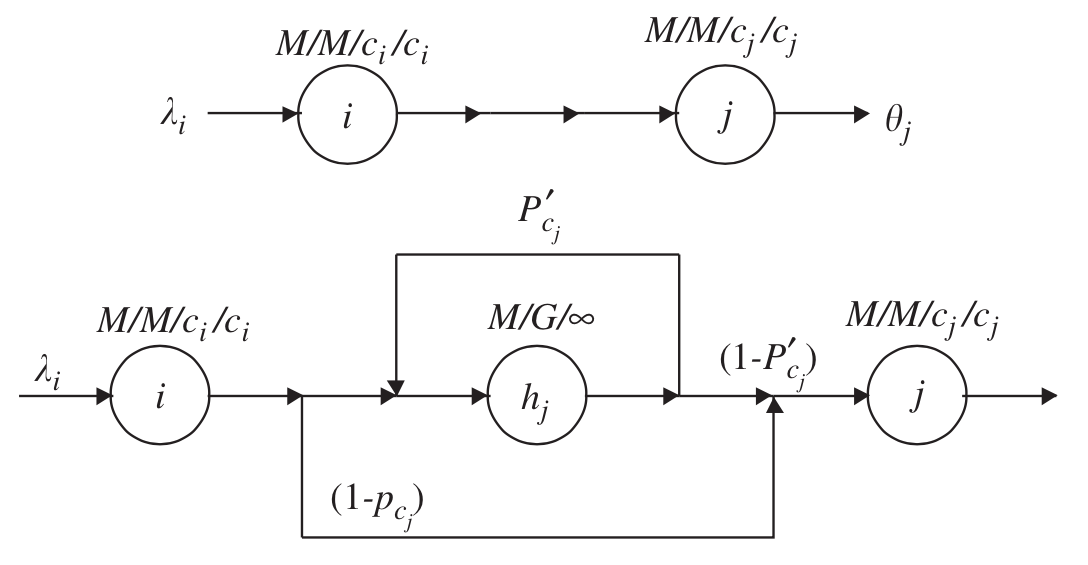
\includegraphics[width=0.4\textwidth]{assets/gem}
\label{fig:gem}
\end{figure}

\subsection{\textbf{Network Performance Optimization}}
\subsubsection{Multi-Objective Optimization}
One commonly used technique is using Multi-Objective Optimization (MOO), which is addressed by Andriansyah \textit{et al.} in \cite{own}. They were the first to use the MOO method, combined with a genetic search algorithm, to evaluate this type of queueing networks. The article tries to optimize two conflicting objectives, minimizing the total number of servers in the system and maximizing the throughput of the system. More servers would increase the throughput, but the cost related to the increase must also be taken into account. The aim of the MOO in this case would be to find the best trade-off between the amount of servers and the throughput. In the next step, a genetic algorithm is used to optimize the MOO function, which is explained in the next section.

\subsubsection{Optimization methodologies}
There exist many optimization methods. In this survey paper, two methodologies are described which have proven to be successful, namely, Powell’s algorithm \cite{powel} and a genetic algorithm approach. Of course, small problems can always be enumerated.
Powell's algorithm can be used for example to find the optimal amount of servers in the system. This conjugate direction method is an algorithm used to find a local minimum of a function. The minimisation of this function is done by executing a bi-directional search along each of the search vectors. A linear combination of these vectors then results in a new search vector which is added to the list. The most helpful vector, the one that played the biggest part in determining the new position, is removed. This algorithm is executed for a certain number of iterations until the result hardly changes any more.
\\\\
Genetic Algorithms (GA) are optimization algorithms to perform an approximate global search relying on the information obtained from the evaluation of several points in the search space and obtaining a population of these points that converges to the optimum through the application of the genetic operators mutation, crossover, selection, and elitism. Each of these operators may be implemented in several different ways, each one of them characterizing a specific instance of the GA. Additionally, convergence of the GA is guaranteed by assigning a fitness to each population member. This approach is successfully been used for both single-objective applications, by Lin \cite{single1} and Calvete $et$ $al.$ \cite{single2}, and for multiple-objective-applications, by Carrano $et$ $al.$ \cite{multi1} and Cruz $et$ $al.$ \cite{article11}.
\section{\textbf{Conclusions and future research}}
The many papers that were mentioned in this survey show that queueing networks with blocking are a challenging research topic. The paper by Andriansyah \textit{et al.} \cite{own} contains the state-of-the-art on how to evaluate these kinds of networks.
To assess the quality of the GEM as an approximate performance evaluation tool, several experiments are conducted. Andriansyah \textit{et al.} conducted experiments using different topologies to both evaluate and optimize the performance of a zero-buffer queueing network \cite{own}.
Afterwards, simulation experiments were set up for the selected cases and the results were compared. The analytical results in \cite{own} seemed very reasonable and acceptable, although they were not always as accurate as desired. For instance, under extreme high utilization rates, that is, heavy traffic and quite a few servers. Nonetheless in the literature, the GEM has proven to be a valuable approach.
\subsection*{\textbf{Future research suggestions}}
In most papers, the throughput is considered as the main performance measure. It would be interesting to evaluate other measures such as cycle time and work-in-process. Another topic for future research is the study of networks with cycles, as many important industrial systems have loops.

%----------------------------------------------------------------------------------------
%	REFERENCE LIST
%----------------------------------------------------------------------------------------
\begin{thebibliography}{9}

\bibitem{extrahillier} %15
  F. Hillier and R. Boling. Finite queues in series with exponential or Erlang service times: a numerical approach. \textit{Operations Research}, vol. 15, no. 2, pp. 286-303, 1967.
% http://web.a.ebscohost.com/ehost/pdfviewer/pdfviewer?sid=d877a955-5433-4b9d-8522-323f9f9d4a32%40sessionmgr4005&vid=1&hid=4204

\bibitem{article2} %2
  D. Hildebrand. On the capacity of tandem server, finite queue, service systems. \textit{Operations Research}, vol. 16, no. 1, pp. 72-82, 1968.
% http://www.jstor.org/stable/168403?seq=1

\bibitem{article20} %13
  F. S. Hillier and K. C. So. The assignment of extra servers to stations in Tandem Queueing systems with small or no buffers. \textit{Performance Evaluation}, vol. 10, no. 3, pp. 219-231, 1989.
% http://www.sciencedirect.com/science/article/pii/0166531689900126

\bibitem{article7} %5
  S. Jain and J. M. Smith. Open finite queueing networks with M/M/C/K parallel servers. \textit{Computers \& Operations Research}, vol. 21, no. 3, pp. 297-317, 1994. 
% http://ac.els-cdn.com/0305054894900922/1-s2.0-0305054894900922-main.pdf?_tid=c5a067e4-6476-11e4-ac34-00000aacb362&acdnat=1415142381_30eefedf1f341b3825981b2e0da5e6e4

\bibitem{article16} %12
  C. Bouras, J. Garofalakis, P. Spirakis and V. Triantafillou. An analytical performance model for multistage interconnection networks with finite, infinite and zero length buffers. \textit{Performance Evaluation}, vol. 34, no. 3, pp. 169-182, 1998.
% http://www.sciencedirect.com/science/article/pii/S0166531698000352

\bibitem{article15} %11
  S. Andradottir, H. Ayhan and D.G. Down. Server assignment policies for maximizing the steady-state throughput of finite queueing systems. \textit{Management Science}, vol. 47, no. 10, pp. 1421-1439, 2001.
% http://pubsonline.informs.org/doi/abs/10.1287/mnsc.47.10.1421.10262

\bibitem{article13} %9
J. M. Smith and F. R. B. Cruz. The buffer allocation problem for general finite buffer queueing networks. \textit{IIE Transactions}, vol. 37, pp. 343–365, 2004.
% ftp://plutao.est.ufmg.br/pub/fcruz/pub/iie.pdf

\bibitem{article21} %14
C. Osorio and M. Bierlaire. An analytic finite capacity queueing network model capturing the propagation of congestion and blocking. \textit{European Journal of Operational Research}, vol. 196, no. 3, pp. 996-1007, 2009.
% http://www.sciencedirect.com/science/article/pii/S0166531698000352

\bibitem{article3} %3
T. Van Woensel, R. Andriansyah, F.R.B. Cruz, J.M. Smith and L. Kerbache. Buffer and server allocation in general multi-server queuing networks. \textit{International Transactions in Operational Research}, vol. 17, no. 2,  pp. 257-286, 2010.
% ftp://est.ufmg.br/pub/fcruz/pub/bcap.pdf

\bibitem{article4} %4
J. M. Smith, F. R. B. Cruz and T. van Woensel. Topological network design of general, finite, multi-server queueing networks. \textit{European Journal of Operational Research}, vol. 201, no. 2, pp. 427-441, 2010.
% http://www.sciencedirect.com/science/article/pii/S0377221709001489

\bibitem{article11} %8
F. R. B. Cruz, T. Van Woensel, and J. M. Smith. Buffer and throughput trade-offs in M/G/1/K queueing networks: a bicriteria approach. \textit{International Journal of Production Economics}, vol. 125, no. 2, pp. 224–234, 2010.
% http://www.sciencedirect.com/science/article/pii/S0925527310000836)

\bibitem{own} %17
R. Andriansyah, T. van Woensel, F. R. B. Cruz, and L. Duczmal. Performance optimization of open zero-buffer multi-server queueing networks, \textit{Computers \& Operations Research}, vol. 37, no. 8, pp. 1472-1487, 2010.
% http://www.sciencedirect.com/science/article/pii/S0305054809002913

\bibitem{article1} %1
  M. H. Yarmand and D. G. Down. Server allocation for zero buffer tandem queues. \textit{European Journal of Operational Research}, vol. 230, no. 3, pp. 596-603, 2013. 
% http://www.sciencedirect.com/science/article/pii/S0377221713004281

\bibitem{article9} %6
  F. R. B. Cruz and T. van Woensel. Finite Queueing Modelling and Optimization: A Selected Review. \textit{Journal of Applied Mathematics}, vol. 2014,  no. 374962, pp. 1-11, 2014.
% http://www.hindawi.com/journals/jam/2014/374962/

\bibitem{article14} %10
  J. M. Smith. System capacity and performance modelling of finite buffer queueing networks. \textit{International Journal of Production Research}, vol. 12, no. 11, pp. 3125-3163, 2014.
% http://phdtree.org/pdf/41297998-system-capacity-and-performance-modelling-of-finite-buffer-queueing-networks/

\bibitem{extracruz} %16
  F. R. B. Cruz, G. Kendall, L. While, A. R. Duarte and N. L. C. Brito. Throughput Maximization of Queueing Networks with Simultaneous Minimization of Service Rates and Buffers. \textit{Mathematical Problems in Engineering}, vol. 2012, no. 692593, pp. 1-19, 2012.
% http://www.hindawi.com/journals/mpe/2012/692593/

\bibitem{closed1} %24
	W. Whitt. Open and closed models for networks of queues. \textit{AT\&T Bell Laboratories Technical Journal}, vol. 63, no. 9, pp. 1911-1979, 1984.
	
\bibitem{mixed} %23
	S. Balsamo, V. de Nitto Personé and R. Onvural. Analysis of Queueing Networks with Blocking. \textit{Kluwer Academic Publishers}, Dordrecht, The Netherlands, 2001.	
	
\bibitem{compblocks} %19
    R.O. Onvural and H.G. Perros. On equivalencies of blocking mechanisms in queueing networks with blocking. \textit{Operations Research Letter}, vol. 5, no. 6, pp. 293-298, 1986.

\bibitem{blocking} %22
	Y. Dallery and S. B. Gershwin. Manufacturing flow line systems: a review of models and analytical results. \textit{Queueing Systems}, vol. 12, no. 1-2, pp. 3-94, 1992.

\bibitem{bbs} %20
	Y. Frein Y and Y. Dallery. Analysis of cyclic queueing networks with finite buffers and blocking before service. \textit{Performance Evaluation}, vol. 10, no. 3, pp. 197-210, 1989.

\bibitem{rs} %21
	S. Matteo. Mean value analysis of product form solution queueing networks with repetitive service blocking. \textit{Performance Evaluation}, vol. 36-37, pp. 19-33, 1999.
	
\bibitem{productform} %27
	H. G. Perros. Queueing networks with blocking: a bibliography. \textit{ACM Sigmetrics}, vol. 12, pp. 8-12, 1984.

\bibitem{gem} %28
	L. Kerbache, J. M. Smith. Asymptotic behavior of the expansion method for open finite queueing networks. \textit{Computers \& Operations Research}, vol. 15, no. 2, pp. 157-69, 1988.

\bibitem{powel} %29
	M. J. D. Powell. An efficient method for finding the minimum of a function of several variables without calculating derivatives. \textit{The Computer Journal}, vol. 7, pp. 155-162, 1964.
	
\bibitem{single1} %30
	F.-T. Lin. Solving the knapsack problem with imprecise weight coefficients using genetic algorithms. \textit{European Journal of Operational Research}, vol. 185, no. 1, pp. 133-145, 2008.
\bibitem{single2} %31
	H. I. Calvete, C. Gale, and P. M. Mateo. A new approach for solving linear bilevel problems using genetic algorithms. \textit{European Journal of Operational Research}, vol. 188, no. 1, pp. 14-28, 2008.
\bibitem{multi1} %32
	E. G. Carrano, L. A. E. Soares, R. H. C. Takahashi, R. R. Saldanha, and O. M. Neto. Electric distribution network multiobjective design using a problem-specific genetic algorithm. \textit{IEEE Transactions on Power Delivery}, vol. 21, no. 2, pp. 995-1005, 2006
	
%\bibitem{article10} %7
%J. M. Smith, F. R. B. Cruz and T. Van Woensel. Optimal server allocation in general, finite, multi-server queueing networks. \textit{Applied Stochastic Models in Business and Industry}, vol. 26, no. 6, pp. 705–736, 2010.
% http://www.researchgate.net/publication/227652730_Optimal_server_allocation_in_general_finite_multiserver_queueing_networks


%
%\bibitem{extra1} %18
%	L. Kerbache and J. M. Smith. The generalized expansion method for open finite queueing networks. \textit{European Journal of Operational Research}, vol. 32, no. 3, pp. 448-461, 1987.
%


%
%\bibitem{closed2} %25
%	 J. M. Smith. Optimal workload allocation in closed queueing networks with state dependent queues. \textit{Annals of Operations Research}, 2013.


\end{thebibliography}

%----------------------------------------------------------------------------------------

\end{multicols}

\end{document}
